\ifx\mainfile\undefined
%  ========================================================================
%  Copyright (c) 2006-2011 The University of Washington
%
%  Licensed under the Apache License, Version 2.0 (the "License");
%  you may not use this file except in compliance with the License.
%  You may obtain a copy of the License at
%
%      http://www.apache.org/licenses/LICENSE-2.0
%
%  Unless required by applicable law or agreed to in writing, software
%  distributed under the License is distributed on an "AS IS" BASIS,
%  WITHOUT WARRANTIES OR CONDITIONS OF ANY KIND, either express or implied.
%  See the License for the specific language governing permissions and
%  limitations under the License.
%  ========================================================================
%
 
\documentclass [11pt, twoside] {uwthesis}

\usepackage{color}
\usepackage{url}
\usepackage{amsmath}
\usepackage{amsfonts}
\usepackage[bookmarks,
	hidelinks,
	plainpages=false,
	pdfpagelabels,
	pagebackref=true,
            ]{hyperref}
\renewcommand*{\backref}[1]{}% for backref < 1.33 necessary
\renewcommand*{\backrefalt}[4]{%
  \ifcase #1 %
    (No citations.)%
  \or
    (Cited on page #2.)%
  \else
    (Cited on pages #2.)%
  \fi
}

\newcommand{\biburl}[1]{{\tt<}\url{#1}{\tt>}}

\hypersetup{%
pdfauthor = {Daniel Chaim Halperin},
pdftitle = {Simplifying the Configuration of 802.11 Wireless Networks with Effective SNR},
pdfsubject = {Ph.D. Dissertation},
pdfkeywords = {},
pdfcreator = {University of Washington, Computer Science and Engineering},
pdfproducer = {},
bookmarksopen = {true},
pdfpagelayout = {TwoColumnRight},
}

\usepackage{footnotebackref}
%%%%%%%%%%%%%%%%%%%%%%%%%%%%%%%%%%%%%%%%%%%%%%%%%%%%%%
%%%        Formatting sections                     %%%
%%%%%%%%%%%%%%%%%%%%%%%%%%%%%%%%%%%%%%%%%%%%%%%%%%%%%%
\newcommand{\algref}[1]{Algorithm~\ref{#1}}
\newcommand{\chapref}[1]{Chapter~\ref{#1}}
\renewcommand{\eqref}[1]{Equation~\ref{#1}}
\newcommand{\figref}[1]{Figure~\ref{#1}}
\newcommand{\secref}[1]{\S\ref{#1}}
\newcommand{\tabref}[1]{Table~\ref{#1}}
\newcommand{\heading}[1]{\vspace{4pt}\noindent\textbf{#1}}
\newcommand{\topheading}[1]{\noindent\textbf{#1}}
\newcommand{\noheading}[0]{\vspace{4pt}\noindent}

%%%%%%%%%%%%%%%%%%%%%%%%%%%%%%%%%%%%%%%%%%%%%%%%%%%%%%
%%%        XXX and other warnings                  %%%
%%%%%%%%%%%%%%%%%%%%%%%%%%%%%%%%%%%%%%%%%%%%%%%%%%%%%%
\newcommand{\xxx}[1]{\textit{\color{red}XXX #1}}

%%%%%%%%%%%%%%%%%%%%%%%%%%%%%%%%%%%%%%%%%%%%%%%%%%%%%%
%%%        Units                                   %%%
%%%%%%%%%%%%%%%%%%%%%%%%%%%%%%%%%%%%%%%%%%%%%%%%%%%%%%
\usepackage{xspace}
\newcommand{\unitsep}{\texorpdfstring{\,}{ }}
\def\unit#1{% from: http://www.tex.ac.uk/cgi-bin/texfaq2html?label=csname "Defining a macro from an argument"
  \expandafter\def\csname #1\endcsname{\unitsep\text{#1}\xspace}%
}
\def\varunit#1#2{% from: http://www.tex.ac.uk/cgi-bin/texfaq2html?label=csname "Defining a macro from an argument"
  \expandafter\def\csname #1\endcsname{\unitsep\text{#2}\xspace}%
}
\unit{GHz}
\unit{MHz}
\unit{kHz}
\unit{Gbps}
\unit{Mbps}
\unit{KB}
\unit{dB}
\unit{dBi}
\unit{dBm}
\unit{W}
\unit{mW}
\varunit{uW}{$\mu$W}
\unit{ms}
\varunit{us}{$\mu$s}
\unit{h}
\unit{m}
\unit{s}
\unit{km}
\unit{cm}
\unit{mm}
\varunit{mmsq}{mm$^\text{2}$}
\varunit{insq}{in$^\text{2}$}
\newcommand{\degree}{\ensuremath{^\circ}\xspace}
\newcommand{\degrees}{\degree}
%%%%%%%%%%%%%%%%%%%%%%%%%%%%%%%%%%%%%%%%%%%%%%%%%%%%%%%%%%%%%%%%%%%%%%%%%%%%%%%%%%%%%%
% Euler for math | Palatino for rm | Helvetica for ss | Courier for tt
%
% From: http://www.tug.org/mactex/fonts/LaTeX_Preamble-Font_Choices.html
%%%%%%%%%%%%%%%%%%%%%%%%%%%%%%%%%%%%%%%%%%%%%%%%%%%%%%%%%%%%%%%%%%%%%%%%%%%%%%%%%%%%%%
\renewcommand{\rmdefault}{ppl} % rm
\usepackage[scaled]{helvet} % ss
\usepackage{courier} % tt
\usepackage{eulervm} % a better implementation of the euler package (not in gwTeX)
\normalfont
\usepackage[T1]{fontenc}
%%%%%%%%%%%%%%%%%%%%%%%%%%%%%%%%%%%%%%%%%%%%%%%%%%%%%%%%%%%%%%%%%%%%%%%%%%%%%%%%%%%%%%

%%%%%%%%%%%%%%%%%%%%%%%%%%%%%%%%%%%%%%%%%%%%%%%%%%%%%%
%%%        Figures                                 %%%
%%%%%%%%%%%%%%%%%%%%%%%%%%%%%%%%%%%%%%%%%%%%%%%%%%%%%%
\usepackage{graphicx}
% Caption package both lets you set the spacing between figure and caption
% and also makes the \figref{} point to the right place.
\usepackage[font=bf,aboveskip=6pt,belowskip=-4mm]{caption}
% Allow subfigures, make them bold
\usepackage[bf,BF,small]{subfigure}
% List of figures
\setcounter{lofdepth}{2}  % Print the chapter and sections to the lot

%%%%%%%%%%%%%%%%%%%%%%%%%%%%%%%%%%%%%%%%%%%%%%%%%%%%%%
%%%        Lists with reduced spacing              %%%
%%%%%%%%%%%%%%%%%%%%%%%%%%%%%%%%%%%%%%%%%%%%%%%%%%%%%%
\usepackage{enumitem}

%%%%%%%%%%%%%%%%%%%%%%%%%%%%%%%%%%%%%%%%%%%%%%%%%%%%%%
%%%        Fancy tables                            %%%
%%%%%%%%%%%%%%%%%%%%%%%%%%%%%%%%%%%%%%%%%%%%%%%%%%%%%%
\usepackage{tabulary}
\usepackage{booktabs}

%%%%%%%%%%%%%%%%%%%%%%%%%%%%%%%%%%%%%%%%%%%%%%%%%%%%%%
%%%        Formatting techniques/tools/etc.        %%%
%%%%%%%%%%%%%%%%%%%%%%%%%%%%%%%%%%%%%%%%%%%%%%%%%%%%%%
\newcommand{\term}[1]{\texttt{#1}}

\begin{document}
 
\textpages
\setcounter{chapter}{7} % Set to n-1!
\fi
%%%%%%%%%%%%%%%%%%%%%%%%%%%%%%%%%%

\cleardoublepage
\chapter{Further Applications of Effective SNR}
\label{chap:esnr_eval}

In the previous chapter, we defined the Effective SNR and showed that it can accurately predict packet delivery for 802.11 rates. In this chapter, we explore applications of Effective SNR to various problems of wireless links and wireless networks.

\begin{table}[htp]
	\centering
	\begin{tabular}{lc}
	\toprule
		\textbf{Application of Effective SNR} & \textbf{Status} \\
	\midrule
		Bitrate/MCS selection & \cite{Halperin_ESNR}\\
		Channel width selection & \cite{Halperin_ESNR}\\
		Antenna selection & \cite{Halperin_ESNR}\\
		Power control & \cite{Halperin_ESNR}\\
		Channel selection & \secref{sec:esnr_chansel}\\
		AP selection & \secref{sec:esnr_apsel}\\
		Path selection/BSS selection in WDS & \secref{sec:esnr_pathsel}\\
		Interference planning \\
		Partial packet recovery/FEC & \cite{Bhartia_FreqDiv}\\
		Beamforming \\
		Multicast rate selection \\
	\bottomrule
	\end{tabular}
	\caption[A variety of applications of Effective SNR]{\label{tab:esnr_uses}A variety of applications of Effective SNR\@.}
\end{table}

\tabref{tab:esnr_uses} shows a list of several potential applications of Effective SNR\@. These range from optimizing various parameters of a single Wi-Fi link, such as the MCS or antenna set used, to coordinating many 802.11 nodes in a dense wireless network. Additionally, we identify applications that can be implemented by looking at other aspects of the Channel State Information in \tabref{tab:csi_uses}. These provide useful primitives that can enable systems to adapt behavior based on the location and movement of the user. Combined, we believe these form the critical building blocks for dense 802.11 networks.

\begin{table}[htp]
	\centering
	\begin{tabular}{lc}
	\toprule
		\textbf{Application of CSI} & \textbf{Status} \\
	\midrule
		Mobility classification & \secref{sec:esnr_mobility}\\
		Indoor localization \\
	\bottomrule
	\end{tabular}
	\caption[A variety of applications of Channel State Information]{\label{tab:csi_uses}A variety of applications of Channel State Information.}
\end{table}

In this chapter, we explore CSI and Effective SNR approaches to implementing four of the above applications.

%%%%%%%%%%%%%%%%%%%%%%%%%%%%%%%%%%%%%%%%%%%%%%%%%%%%%%%%%%%%%%%%%%%%%%%%%%%%%%%%%%%%%%%%%%%%%%%%%%%%%%%%%%%%%%%%%%%%%%%%%%%%%%%%%%%%%%%%%
%%%%%%%%%%%%%%%%%%%%%%%%%%%%%%%%%%%%%%%%%%%%%%%%%%%%%%%%%%%%%%%%%%%%%%%%%%%%%%%%%%%%%%%%%%%%%%%%%%%%%%%%%%%%%%%%%%%%%%%%%%%%%%%%%%%%%%%%%
\section{Channel Selection}\label{sec:esnr_chansel}
Using the new Wi-Fi Direct standard, 802.11 devices that wish to send data directly (instead of through the access point as in 802.11 infrastructure mode) can create a peer-to-peer link. Depending on the amount of interference in the network (e.g., from other clients of the access point) and the quality of the link between the two devices, they may wish to move the link to a different operating channel in order to improve performance. This is one example of the \emph{channel selection} problem: to quickly choose the best operating frequency for a pair of nodes to communicate. In this section, I define the ``best'' channel to be the channel that provides the highest throughput in the absence of interferers.

The channel selection problem is similar to the access point selection problem, and has a similar algorithmic solution (\algref{alg:chan_sel_basic}). It can use the same \fcall{GetMetric} functions for Packet SNR (\algref{alg:snr_link_metric}) and Effective SNR (\algref{alg:eff_snr_link_metric}). The primary difference is a reordering of the parameters: rather than a fixed receiver with fixed channel choosing between multiple senders, a fixed sender and receiver must choose between multiple channels.

%%%%%%%%%%%%%%%%%%%%%%%%%%%%%%%%%%%%%%%%%%%%%%%%
\begin{algorithm}[thp]
\caption{\label{alg:chan_sel_basic}\fcall{ChannelSelection(Channel Set $C$, Sender $s$, Receiver $r$)}}
\begin{algorithmic}[1]
\FORALL{$c \in C$}
\STATE Both $s$ and $r$ switch to channel $c$
\STATE Compute the channel metric $m_c$ using $\fcall{GetMetric}(s,r)$
\ENDFOR
\RETURN $\argmax_{c\in C} m_c$ \hfill \COMMENT{choose the channel with the best metric}
\end{algorithmic}
\end{algorithm}
%%%%%%%%%%%%%%%%%%%%%%%%%%%%%%%%%%%%%%%%%%%%%%%%

%%%%%%%%%%%%%%%%%%%%%%%%%%%%%%%%%%%%%%%%%%%%%%%%%%%%%%%%%%%%%%%%%%%%%%%%%%%%%%%%%%%%%%%%%%%%%%%%%%%%%%%%%%%%%%%%%%%%%%%%%%%%%%%%%%%%%%%%%
\subsection{Characterization of 802.11 Channels}
To start my investigation of channel selection algorithms, I first measured how the operating frequency affects 802.11n links in practice.

As in \secref{sec:esnr_apsel}, I filtered the data to the 11 channels in the 5\GHz band for which there are not co-channel university APs. (Note that channel selection generally makes sense \emph{within} one frequency band. Selection across bands is trivial: due to better antenna gain and Friis' Law effects a 2.4\GHz channel has typically 10\dB--15\dB stronger SNR than a 5\GHz channel for the same nodes.) I further eliminated from consideration any pairs of devices that didn't obtain at least 6.5\Mbps throughput on at least 3 of the 11 channels. This left 201 unidirectional links, approximately a third of the $24*23=552$ unidirectional links in the testbed.

\begin{figure}[t]
	\centering
	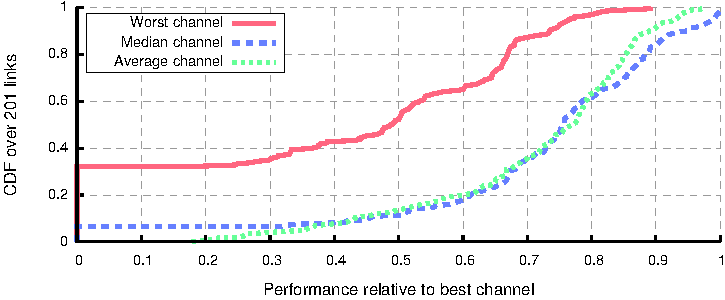
\includegraphics[width=\textwidth]{figures/applications/chan_sel_rel_diff.pdf}
	\caption[The relative difference in throughput over 802.11n channels]{\label{fig:chan_sel_rel_diff}The relative difference in throughput over 802.11n channels.}
\end{figure}

\begin{figure}[t]
	\centering
	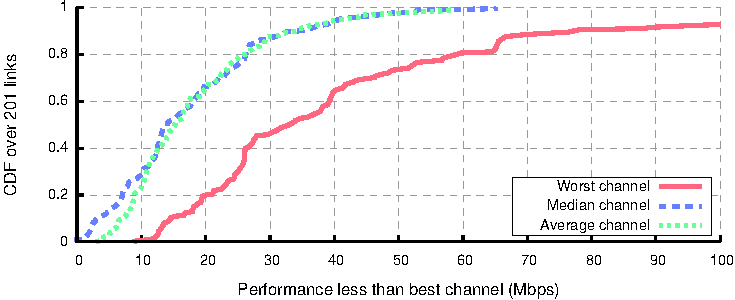
\includegraphics[width=\textwidth]{figures/applications/chan_sel_tpt_diff.pdf}
	\caption[The absolute difference in throughput over 802.11n channels]{\label{fig:chan_sel_tpt_diff}The absolute difference in throughput over 802.11n channels.}
\end{figure}

\subsubsection{Results}
\figref{fig:chan_sel_rel_diff} and \figref{fig:chan_sel_tpt_diff} show how the throughput of the worst, median, and average channels compares to the best channel for these links. Note that because the channel set is fixed and independent of connectivity, the worst channel might deliver no throughput at all---unlike AP selection, in which the client was choosing from only those nodes that responded to its probe. About a third of the links had at least one such channel.

These figures demonstrate that the choice of channel can dramatically impact performance. \figref{fig:chan_sel_rel_diff} shows that the worst channel offers less than half of the best throughput for more than half the links. In absolute terms, this difference can be quite large: the worst channel is a median 33\Mbps worse than the best channel, and for a few links (about 7\%) the difference is more than 100\Mbps. For these links, some channel will deliver no packets at all, while another delivers packets at nearly the maximum bitrate. An unlucky choice of channel can cripple performance and result in little to no throughput.

The median and average channels perform about equivalently in our testbed, and even these are significantly worse. These channels yield less than half the optimal throughput for 15\% of the links and for only one third of links do these come within 80\% of the best throughput. These figures show that for very few links do most channels perform about the same, and the median or average channel is 15\Mbps worse than the best channel for most links, and the gap is larger than 25\Mbps for 20\% of links.

\subsubsection{Signal Strength Across Channels}
Note that the average/median channels are much closer to optimal in these graphs than were the average/median access points we saw in \figref{fig:ap_sel_rel_diff} and \figref{fig:ap_sel_tpt_diff}. Why should this be the case?

I hypothesized that this effect might arise because channels between the same two devices are likely to have similar total signal strengths (i.e., Packet SNR). When two channels have the same signal strength, the difference in performance would come mainly through subchannel fading effects---and while these subchannel effects can affect link quality significantly, as I showed in \chapref{chap:delivery}, the difference is likely not as much as when comparing access points located tens of meters apart.

To test this hypothesis, I analyzed the Packet SNR versus channel for the 11 channels supported by the IWL5300 in the 2.4\GHz band and the 24 channels in the 5\GHz band.\footnote{I used all channels for these experiments, as external interference does not pose a problem. Accurate SNR measurements require only a single packet to be delivered successfully without interference during the preamble.} I considered only links that had at least 10 packets delivered with consistent SNRs and supported at least 3 channels, for a total or 349 links in the 2.4\GHz band and 253 links in the 5\GHz band.

If different channels have similar signal strengths, the Packet SNR will vary only a few dB across the frequency band. \figref{fig:rssi_vs_freq_24} and \figref{fig:rssi_vs_freq_5} plot the normalized Packet SNR for a given link (Packet SNR across all channels minus the average Packet SNR) against channel. The figures include one grey line per link, and the solid black line in each figure shows the median. We see that, indeed, Packet SNR stays within a few dB of the median for most channels. I believe that the shape of the black line in \figref{fig:rssi_vs_freq_5} shows the natural resonance of the antennas, which is consistently non-uniform across the approximately 600\MHz of spectrum the 5\GHz band covers.

\begin{figure}[htp]
	\centering
	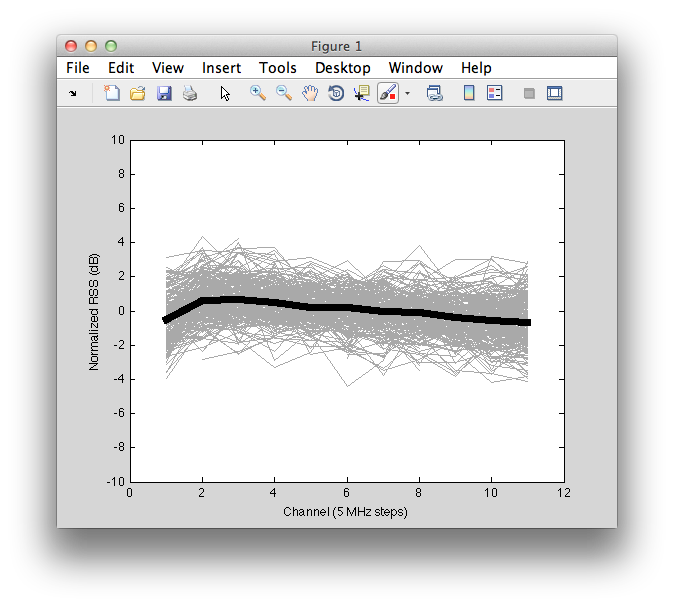
\includegraphics[width=0.6\textwidth]{figures/esnr/rssi_vs_freq_24.png}
	\caption[Normalized Packet SNR versus 2.4\GHz channel for 349 links]{\label{fig:rssi_vs_freq_24}Normalized Packet SNR versus 2.4\GHz channel for 349 links. Solid line shows the median for each channel.}
\end{figure}
\begin{figure}[htp]
	\centering
	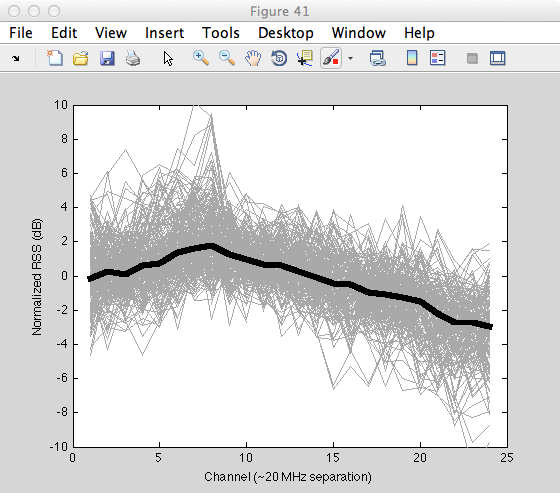
\includegraphics[width=0.6\textwidth]{figures/esnr/rssi_vs_freq_5.png}
	\caption[Normalized Packet SNR versus 5\GHz channel for 253 links]{\label{fig:rssi_vs_freq_5}Normalized Packet SNR versus 5\GHz channel for 253 links. Solid line shows the median for each channel.}
\end{figure}
%\begin{figure}[htp]
%	\centering
%	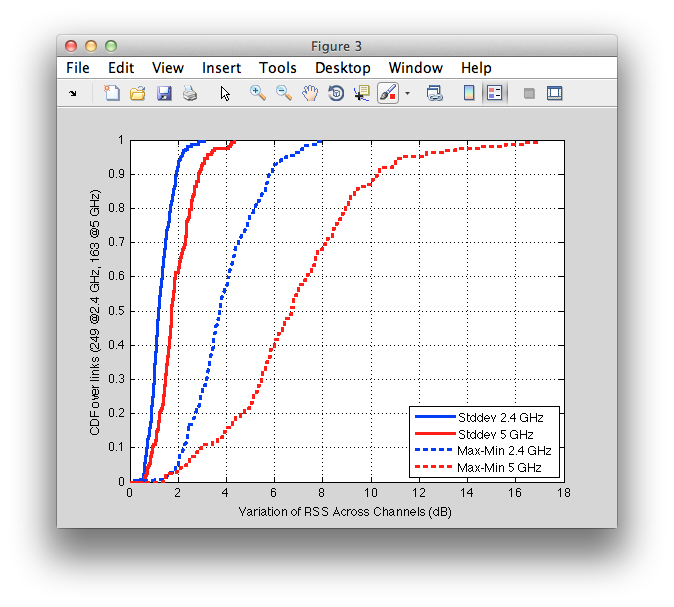
\includegraphics[width=0.6\textwidth]{figures/esnr/rssi_freq_dev.png}
%	\caption{\label{fig:rssi_freq_dev}Standard deviation and max-min spread of Packet SNR across channels within the same band.}
%\end{figure}

From these results, I conclude that a strategy that picks a fixed channel or a random channel will perform significantly worse than a strategy that can identify channels that are likely to offer good performance. Note that this is implicitly the channel selection strategy for strategies that attempt to short-circuit the AP~\cite{Afanasyev_RTSid} used in today's infrastructure networks, because the channel is fixed by the AP. At the same time, because for a fixed link, most channels have roughly the same Packet SNR, fading effects should play a larger role in determining the best channel. This makes the channel selection problem is harder than the AP selection problem, and the solutions may perform slightly worse; however Effective SNR should provide a larger advantage in this case. Having motivated the need for an accurate channel selection algorithm, I present and evaluate different channel selection strategies in the rest of this section.

%%%%%%%%%%%%%%%%%%%%%%%%%%%%%%%%%%%%%%%%%%%%%%%%%%%%%%%%%%%%%%%%%%%%%%%%%%%%%%%%%%%%%%%%%%%%%%%%%%%%%%%%%%%%%%%%%%%%%%%%%%%%%%%%%%%%%%%%%%
%\subsection{Channel Selection Algorithms}
%\algref{alg:chan_sel_basic} is a template for a channel selection algorithm. It takes as input a list of channels to evaluate $C$, and a sender $s$ and receiver $r$ that together define a link. The two nodes hop across channels, using the \fcall{PredictThroughput} function to evaluate the performance of the link on each. The algorithm tracks the best performing channel, labeled $c_{\max}$ and returns that value. (\fcall{ChannelSelection} can also return $\emptyset$ if all channels have zero predicted throughput, but we only consider links that can communicate on at least 1 channel.) Using this template, different channel selection algorithms can be instantiated by providing different implementations of \fcall{PredictThroughput}.
%
%%%%%%%%%%%%%%%%%%%%%%%%%%%%%%%%%%%%%%%%%%%%%%%%%
%\begin{algorithm}[htp]
%\caption{\label{alg:chan_sel_basic}\fcall{ChannelSelection($C, s, r$)}}
%\begin{algorithmic}
%\STATE $t_{\max}\gets 0\Mbps$
%\STATE $c_{\text{best}} \gets \emptyset$
%\FORALL{$c \in C$}
%\STATE Both $s$ and $r$ switch to channel $c$
%\STATE $t \gets \fcall{PredictThroughput($s, r$)}$
%\IF{$t > t_{\max}$}
%	\STATE $t_{\max} \gets t$
%	\STATE $c_{\text{best}} \gets c$
%\ENDIF
%\STATE \textbf{return} $c_{\text{best}}$
%\ENDFOR
%\end{algorithmic}
%\end{algorithm}
%%%%%%%%%%%%%%%%%%%%%%%%%%%%%%%%%%%%%%%%%%%%%%%%%
%
%I consider three different channel selection algorithms in this section. The first is \fcall{ChannelSelectionOPT}, an oracular channel selection algorithm that chooses the optimal channel. For implementation purposes, I instantiate \fcall{ChannelSelectionOPT} by \algref{alg:chan_sel_probe} (\fcall{ProbeChannelThroughput}), which probes all MCSes with MTU-sized packets to determine packet delivery and predicts throughput according to \eqref{eq:prr_throughput}.
%
%%%%%%%%%%%%%%%%%%%%%%%%%%%%%%%%%%%%%%%%%%%%%%%%%
%\begin{algorithm}[tp]
%\caption{\label{alg:chan_sel_probe}\fcall{ProbeThroughput($s, r$)}}
%\begin{algorithmic}
%\STATE $p_0,p_1,\dots,p_{23} \gets 0$
%\STATE $N \gets \text{number of probes at each MCS}$
%\FOR{$i = 1 \dots N$}
%\FOR{$m = 0 \dots 23$}
%\STATE $s$ sends one MTU-sized packet at \mcs{$m$}
%\IF{$s$ receives an ACK from $r$}
%\STATE $p_m \gets p_m + 1$
%\ENDIF
%\ENDFOR
%\ENDFOR
%\STATE $t_{\max}\gets \max \{p_m/N \cdot M(m)\} \text{ over all } m$ \hfill \COMMENT{\eqref{eq:prr_throughput}}
%\STATE \textbf{return} $t_{\max}$
%\end{algorithmic}
%\end{algorithm}
%%%%%%%%%%%%%%%%%%%%%%%%%%%%%%%%%%%%%%%%%%%%%%%%%
%%%%%%%%%%%%%%%%%%%%%%%%%%%%%%%%%%%%%%%%%%%%%%%%%
%\begin{algorithm}[tp]
%\caption{\label{alg:chan_sel_esnr}\fcall{PredictThroughputESNR($s, r$)}}
%\begin{algorithmic}
%\FOR{$m \in \{16, 8, 0\}$}
%\STATE $s$ sends one packet with 0-byte payload at \mcs{$m$}
%\STATE $r$ computes the Effective SNR values $\rho_\text{eff}$ and returns them along with the ACK
%\IF{$s$ receives an ACK from $r$}
%	\STATE \textbf{return} \fcall{ESNRToThroughput}($\rho_\text{eff}$), $\rho_\text{eff}$ \hfill \COMMENT{$\rho_\text{eff}$ is used to break ties}
%\ENDIF
%\ENDFOR
%\STATE \textbf{return} 0
%\end{algorithmic}
%\end{algorithm}
%%%%%%%%%%%%%%%%%%%%%%%%%%%%%%%%%%%%%%%%%%%%%%%%%
%
%The second algorithm chooses the channel based on RSS, presented in \algref{alg:chan_sel_rss}. In this case, the sender only needs to send a single probe packet (with no payload) in order to measure the RSS on the channel. Since \fcall{RSSToThroughput} is monotonically increasing in RSS, this algorithm is equivalent to selecting the channel with the maximum RSS\@.
%
%The third algorithm chooses the channel based on the Effective SNR, presented in \algref{alg:chan_sel_esnr}. Here, the sender sends probes (with no payload) with decreasing numbers of spatial streams to enable the receiver to collect a maximal CSI measurement. The receiver then sends the computed Effective SNR values back to the sender, which uses them to predict the best rate.
%
%I evaluate these three algorithms in the next section.

%%%%%%%%%%%%%%%%%%%%%%%%%%%%%%%%%%%%%%%%%%%%%%%%%%%%%%%%%%%%%%%%%%%%%%%%%%%%%%%%%%%%%%%%%%%%%%%%%%%%%%%%%%%%%%%%%%%%%%%%%%%%%%%%%%%%%%%%%
\subsection{Channel Selection Accuracy}
I evaluate Packet SNR and Effective SNR-based channel selection algorithms based on \algref{alg:chan_sel_basic} and using the link metric functions described in \algref{alg:snr_link_metric} (Packet SNR) and \algref{alg:eff_snr_link_metric} (Effective SNR).

\figref{fig:chan_sel_ratio_opt} shows the performance relative to the optimal algorithm when using Effective SNR or Packet SNR to choose between channels, using the same format as I used for access point selection in \figref{fig:ap_sel_ratio_opt}. Again, we see that both algorithms perform well, though Effective SNR is a better predictor of application performance. Effective SNR chooses an optimal channel for 121 links (60\%), whereas Packet SNR is optimal for only 71 links (35\%). The Effective SNR-based algorithm is within 90\% of optimal for 168 links (84\%), 80\% for 181 links (90\%), and 70\% for 191 links (95\%). In contrast, maximizing the Packet SNR only gets within 90\% of optimal for 112 links (56\%).

\begin{figure}[p]
	\centering
	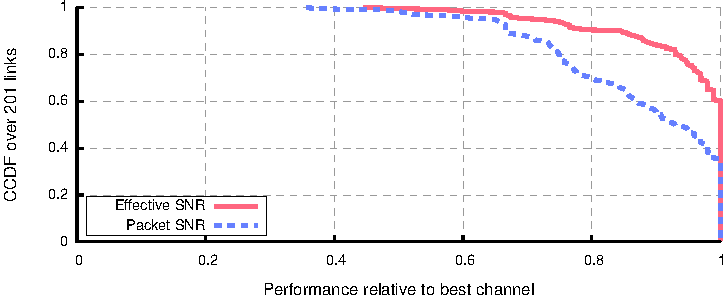
\includegraphics[width=\textwidth]{figures/applications/chan_sel_ratio_opt.pdf}
	\caption[Channel selection algorithm performance relative to Optimal]{\label{fig:chan_sel_ratio_opt}Channel selection algorithm performance relative to an optimal algorithm.}
\end{figure}
\begin{figure}[p]
	\centering
	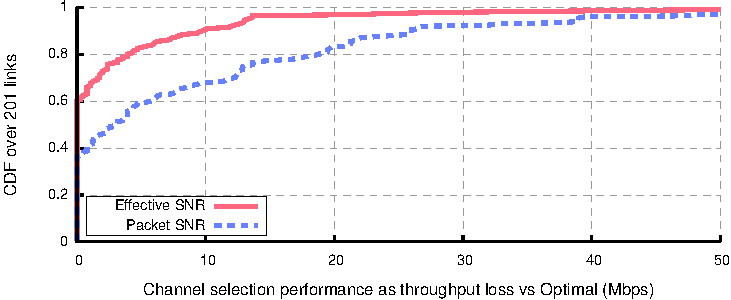
\includegraphics[width=\textwidth]{figures/applications/chan_sel_diff_opt.pdf}
	\caption[Channel selection algorithm performance loss from Optimal]{\label{fig:chan_sel_delta_opt}Channel selection algorithm performance loss from optimal algorithm.}
\end{figure}
\begin{figure}[p]
	\centering
	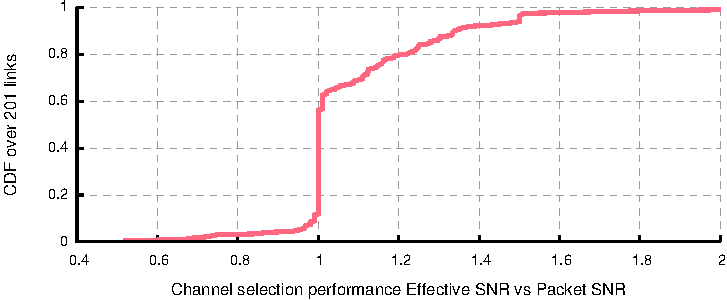
\includegraphics[width=\textwidth]{figures/applications/chan_sel_ratio.pdf}
	\caption[Channel selection algorithm performance with Effective SNR relative to Packet SNR]{\label{fig:chan_sel_ratio}Channel selection performance with Effective SNR relative to Packet SNR.}
\end{figure}

Next, I compare the absolute performance loss of the channel selection algorithms in \figref{fig:chan_sel_delta_opt}. Again, the area over the curves represents the performance lost by each algorithm. This area is 3.3$\times$ larger for the Packet SNR-based selection algorithm, showing that Effective SNR is significantly more accurate. This difference translates to about 9\Mbps faster links when selecting channels via the Effective SNR.

Finally, \figref{fig:chan_sel_ratio} shows the ratio of the performance of the channels selected by Effective SNR and Packet SNR. Recall that a ratio larger than 1 means that Effective SNR chose a faster operating channel. The algorithms choose channels with equal performance for 82 (41\%) of the 201 links, while the Effective SNR-based algorithm chooses a better channel for 94 (47\%) links and the Packet SNR-based algorithm for the remaining 25 (12\%). Additionally, the gains from Effective SNR are much larger than its losses: the Packet SNR strategy chooses a channel that performs 20\% better than the Effective SNR-selected channel for only 4/25 (16\%) links when its channel is better, while Effective SNR chooses a 20\% better channel for 50/94 (53\%) of cases. In other words, the Effective SNR channel selection algorithm is more likely to pick a better channel by a factor of about 4 (94/25), and this difference is more likely to be significant by a factor of about 3 (53\%/16\%).

\heading{Summary.}
These results shows that both Effective SNR- and Packet SNR-based channel selection strategies perform well in my testbed. However, the Effective SNR channel selection strategy is significantly more accurate: it chooses an optimal channel for 70\% more links, it offers about 9\Mbps more per link when selecting suboptimal channels, and it is more likely to choose a better channel than a worse channel by a factor of 4.

Note also that, as hypothesized above, the accuracy of both channel selection algorithms is reduced relative to access point selection. Whereas Effective SNR chose an optimal AP for more than 80\% of clients, it indicates an optimal channel for only 60\% of links; the Packet SNR results exhibit similar a similar decline. This confirms that the similarity of channels leads to more ambiguity when choosing between them. Additionally, the benefits of Effective SNR relative to Packet SNR are larger for channel selection than they were for AP selection. Since most channels have similar Packet SNRs, the real reason for the improvement performance is that my model can accurately assess the impact of subchannel fading effects.

%%%%%%%%%%%%%%%%%%%%%%%%%%%%%%%%%%%%%%%%%%%%%%%%%%%%%%%%%%%%%%%%%%%%%%%%%%%%%%%%%%%%%%%%%%%%%%%%%%%%%%%%%%%%%%%%%%%%%%%%%%%%%%%%%%%%%%%%%%
%\subsection{\xxx{Further Evaluations?}}
%\heading{Channel discrimination.}
%\xxx{how many channels do we need to look at to get good performance?} \figref{fig:rel_diff_draws} shows that, depending on how close to optimal you want to be, need to look at 5, 10, or 15 of the 24 channels in 5\GHz band. If we can evaluate the rate offered by a channel quickly, we can look at more channels in the same amount of time to pick the best rate.
%
%\begin{figure}[htp]
%	\centering
%	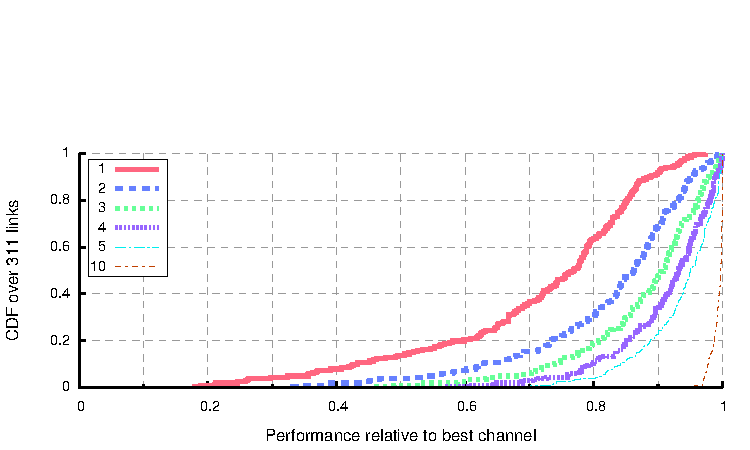
\includegraphics[width=\textwidth]{figures/applications/chan_sel_rel_diff_draws.pdf}
%	\caption[The expected rate after choosing the best of $k$ 802.11n channels]{\label{fig:rel_diff_draws}The expected rate after choosing the best of $k$ 802.11n channels.}
%\end{figure}
%
%\heading{Performance.} \xxx{given time to hop $\mathcal{O}$(1\ms), time to execute a CSI probe $\mathcal{O}$(500\us), and time to execute a rate probe (unknown), how many channels can we look at in $T$ time? Reference \figref{fig:rel_diff_draws} to see what fraction of optimal this enables.}
%
%\heading{Completion Time.} \xxx{The difference between the Effective SNR and the SNR is a proxy for how ``good'' a channel is, based on how flat it is. Given that RSS is similar across channels, the flattest channel will likely offer the best rate. Can we use this to detect a good channel and stop looking early?}
%%%%%%%%%%%%%%%%%%%%%%%%%%%%%%%%%%%%%%%%%%%%%%%%%%%%%%%%%%%%%%%%%%%%%%%%%%%%%%%%%%%%%%%%%%%%%%%%%%%%%%%%%%%%%%%%%%%%%%%%%%%%%%%%%%%%%%%%%
\section{AP selection}\label{sec:esnr_apsel}
In a dense network, a new client may need to select its parent from many available repeaters in addition to the network coordinator. In enterprise AP and Wireless Distribution System networks today, clients typically choose the node whose probe response has the highest SNR\@. (\xxx{though there is heaps of related work doing more complex things.}) In dual-band networks, some devices may prefer a 5\GHz AP with slightly lower SNR, as long as it exceeds a minimum threshold, based on the optimistic assumption that interference is lower in the 5\GHz band. Here, we describe a procedure that uses the Effective SNR to improve this decision process and select a good parent.

Normally, a client scanning for a network cycles through the available channels sends a probe request at the lowest rate (including a single stream and 20\MHz channels), and all APs or repeaters in range respond. We propose that the client instead send multiple probes that use the lowest 6.5\Mbps rate, but vary the number of streams and channel width in decreasing order. In this way, the coordinator and all repeaters that measure CSI from the probes can compute the Effective SNR for the uplink. The probe responses can now include the computed Effective SNR to better inform the client's choice. If the client includes its transmit power level in the probe request (or if the responder makes a conservative estimate), then the responder can combine this information with the CSI measured from the probe to compute the Effective SNR for the downlink. It can then send the probe response at a faster rate than the base rate and reduce the overhead of the probe response.

\subsection{Evaluation methodology}
Compare the following strategies:
\begin{figure}[htp]
	\centering
	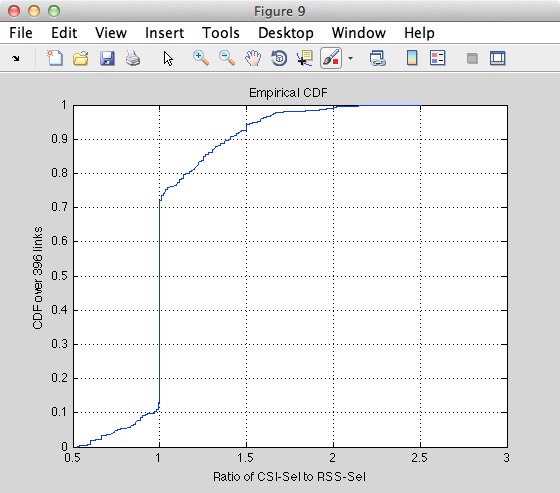
\includegraphics[width=0.6\textwidth]{figures/esnr/ap_sel_ratio.png}
	\caption{\label{fig:ap_sel_ratio}The relative throughput selecting APs by Packet SNR or by Effective SNR\@.}
\end{figure}

\begin{figure}[htp]
	\centering
	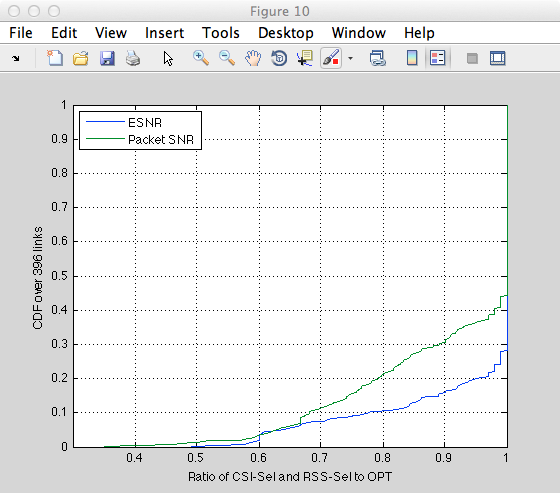
\includegraphics[width=0.6\textwidth]{figures/esnr/ap_sel_ratio_opt.png}
	\caption{\label{fig:ap_sel_ratio_opt}AP selection using Packet SNR or Effective SNR compared to Optimal.}
\end{figure}

\begin{figure}[htp]
	\centering
	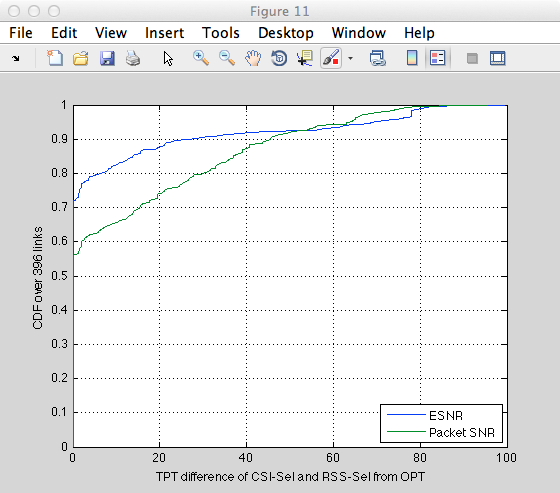
\includegraphics[width=0.6\textwidth]{figures/esnr/ap_sel_delta_opt.png}
	\caption{\label{fig:ap_sel_delta_opt}The difference in throughput using APs selected by Packet SNR or Effective SNR compared to Optimal.}
\end{figure}
\begin{itemize}
\item first AP seen
\item max RSSI
\item max CSI predicted rate
\item max measured rate
\end{itemize}

%%%%%%%%%%%%%%%%%%%%%%%%%%%%%%%%%%%%%%%%%%%%%%%%%%%%%%%%%%%%%%%%%%%%%%%%%%%%%%%%%%%%%%%%%%%%%%%%%%%%%%%%%%%%%%%%%%%%%%%%%%%%%%%%%%%%%%%%%
\section{Path selection}\label{sec:esnr_pathsel}
In the last section, we looked at the benefits of AP selection; we now consider the more general problem of path selection. While today's AP and WDS\footnote{Actually, a WDS client implicitly makes a routing decision when joining the network---which access point it chooses can make a large difference in its connection quality.} networks use tree-structured topologies and have only a single path between any two nodes, a future device-to-device wireless network may offer many paths along which packets can be routed. Research in multi-hop routing for wireless mesh networks~\cite{Bahl_repeater,Rodrig_thesis} has shown that the choice of path can effect a large difference in connection quality.

The practical state of the art in this area is the recent work by Bahl et al.~\cite{Bahl_repeater} on an opportunistic repeater scheme for 802.11a. In this design, when a client with a strong link detects rate anomaly~\cite{Heusse_RateAnomaly}---that is, that its throughput is hurt by a client with a weak link monopolizing airtime---the strong client evaluates whether relaying that client's packets would improve throughout for both. In certain scenarios, they showed that this could improve aggregate performance of the network by 50\%--200\%.

While this solution is practical and effective, the use of 802.11n networks significantly complicates the picture. First, the scheme of Bahl et al.\ uses a link's RSSI to select between the 8 available 802.11a rates. In contrast, as we have shown in \chapref{chap:esnr_intro}, RSSI does not accurately predict the rate for 802.11n links, nor does it enable devices to choose between different MIMO modes. Bahl et al.\ used a homogenous network of single-antenna 802.11a chipsets; the set of devices in 802.11n networks includes those with differing numbers of antennas and asymmetric transmit/receive capabilities. While it is not clear how to handle these challenges via the RSSI, the Effective SNR offers the ability to overcome them. In this section, we evaluate the ability of Effective SNR to deliver the benefits of opportunistic repeaters in 802.11n networks.

Note that the problem of path selection does not differ significantly from that of AP selection, except that when choosing between repeaters (or a direct link) the entire path must be considered rather than merely the last hop.\footnote{For simplicity, we assume that the network diameter is small such that pipelining~\cite{Rodrig_thesis} is of limited benefit, and do not consider schemes that forward along multiple unreliable paths such as ExOR~\cite{Biswas_ExOR}.} Instead, in this section we focus on how 802.11n and heterogeneous devices change the opportunities available from relaying, and whether Effective SNR delivers these improvements.

\subsection{Measurements on 802.11a vs 802.11n}
Denote node in center of testbed as AP, and pick a channel. Consider nodes in decreasing order of RSS: have them associate to the network, then turn into repeaters from which the next node can choose. Assume optimal decisions are made at each step. Compare 1x1, 1x3, and 3x3 versions of this scenario.
\begin{itemize}
\item What is the distribution of distance (\#hops) from each node to AP? [How often is repeating used, and at what scale?]
\item What is the distribution of end-to-end tpt? Of the fraction of max (i.e., 65\Mbps or 195\Mbps)? Of the improvement? [This gets at whether the gains get larger or smaller with various device changes.]
\end{itemize}
Same scenario with randomly assigned 3x3, 2x3, and 1x3 devices. How does heterogeneity affect these results?

\subsection{Measurements of Effective SNR}
Perform the same experiments as described above, this time predicting rate by RSSI and then by Effective SNR\@. (Use this only for topology choice, but assume rate selection finds the correct rate.)

%%%%%%%%%%%%%%%%%%%%%%%%%%%%%%%%%%%%%%%%%%%%%%%%%%%%%%%%%%%%%%%%%%%%%%%%%%%%%%%%%%%%%%%%%%%%%%%%%%%%%%%%%%%%%%%%%%%%%%%%%%%%%%%%%%%%%%%%%
\section{Mobility classification}\label{sec:esnr_mobility}
In wireless systems, simply knowing whether a device is mobile can improve performance and reliability. For example, recent work of Ravindranath et al.\ \cite{Ravindranath_SensorHints} demonstrated a system that improved 802.11a performance on a mobile phone by selecting between different bitrate adaptation algorithms based on whether the device was moving. When the device is static, they use algorithms that can conduct a fine-grained search of the rate space to choose the optimum bitrate. When the device is moving, they use an algorithm that performs a coarser search, but does a better job of tracking a moving optimum. In their experiments, the fine-grained algorithms performed 10\%--30\% better in static scenarios, while the coarse-grained algorithm performed 25\%--75\% better in mobile scenarios.

Detecting mobility can also be used to enhance reliability in networks that support dynamic topology, such as today's cellular phone networks, enterprise Wi-Fi wireless distribution systems (WDSes), and networks that support relaying mechanisms such as described above. By proactively looking for a better AP or relay when the device starts moving, service quality can be improved and downtime reduced. \xxx{find some references about cell handoff, WDS handoff, etc.}

The implementation by Ravindranath et al.\ detected mobility using the accelerometer in a mobile phone. While this technique is accurate and responsive, it has a few disadvantages. The use of an on-board sensor means that detection can only be performed by the mobile client, and thus requires protocol changes to communicate a device's mobile state to the other endpoint of the link, and is not backwards-compatible. Also, this technique can only be implemented on devices that have accelerometers, and requires that this sensor be powered on.

In this section, I explore whether it is possible to classify whether a device is mobile based solely on passively measured RF information. If successful, such an implementation would eliminate all of these drawbacks by requiring no extra hardware and supporting unilateral adoption by either endpoint of the link, including the static device. Ravindranath et al.\ made a preliminary attempt to classify mobility using RSSI, but were not successful. They list three challenges: (1) that RSSI is unstable even for static links in a quiet environment; (2) that RSSI varies by different amounts at different absolute signal strengths, and thus needs to be calibrated; and (3) that RSSI was extremely sensitive to movement in the environment and triggered many false hints. Here, I show that the CSI can overcome these challenges and provide a robust solution.

\subsection{Experimental setup}
I configured a SIMO experiment using a single-antenna laptop as the client device, and several of the testbed nodes as three-antenna monitors. The client sent 100,000 back-to-back short packets using MCS~0 (1 stream, 6.5\Mbps), approximately one packet every 300\us for 20\s. In my initial data collection described here, I took four traces. Two of the traces were taken with a \emph{static} client in the UW CSE Networking Lab and students present, but not moving in the room. I then took a trace with \emph{environmental mobility} in which I left the client static, but waved my hand within a few centimeters of the antenna and then walked around the room and opened doors. Finally, I took a \emph{mobile device} trace in which I picked up the laptop and moved it around within a meter of its original location. Chronologically, the traces were taken in the order described within a 10-minute window, with the second static trace taken last. \xxx{These results are from only a single receiver and a single mobile experiment; I could look at more traces and conduct more experiments to flesh out the results and to address claim (2) above.}

\subsection{Evaluation}
\topheading{Classifying mobility with RSS\@.} \figref{fig:mobility_rssi} shows the RSS in dBm measured by one receiver for these four traces. Each line shows the RSS for one of the three receive antennas. I note several interesting effects visible in these measurements. First, the RSS is actually extremely stable in static scenarios. This deviation from Ravindranath et al.\ is likely attributable to the better calibration of the newer 802.11n hardware we use, compared with older hardware used to run experiments with the MadWiFi driver. Second, though RSS does vary with environmental mobility, the variation is fairly small and mostly limited to the periods of activity directly next to the client---later in the trace, when I moved across the room, the RSS variation decreased to the static scenario. It also appears that the variation is not completely correlated across antennas; in several parts of the trace (e.g., at the beginning and around 10--12\s) one or two experience antennas see variation in RSS while the others do not. Finally, the mobile trace exhibits the RSS variation with the largest magnitude, and shows consistent variation throughout the trace and across all antennas. Based on this visual evidence, I conclude it likely that the static scenario can be identified using RSS, and hypothesize that it may also be possible to distinguish between environmental and device mobility. However, I deferred from exploring this possibility further because, as I will show next, the CSI can conclusively classify a device's activity into these three states.

\begin{figure}[htp]
	\centering
	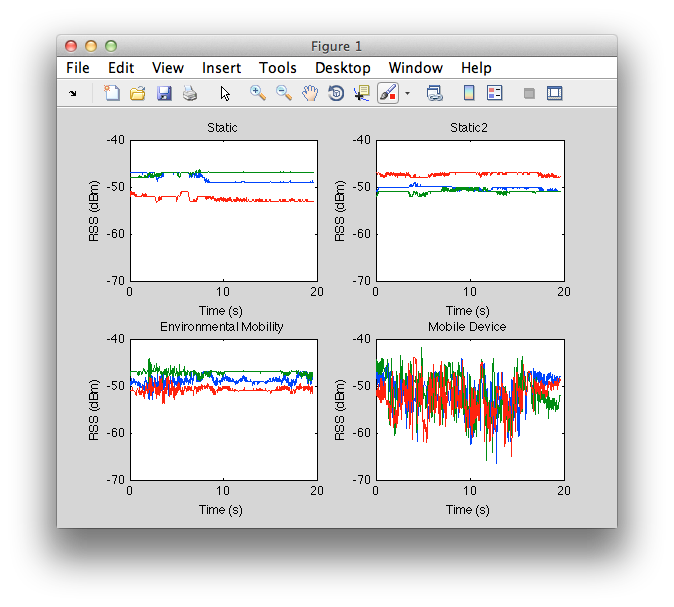
\includegraphics[width=\textwidth]{figures/esnr/mobility_rssi.png}
	\caption{\label{fig:mobility_rssi}RSSI variation in different mobility scenarios.}
\end{figure}

\heading{Classifying mobility with CSI\@.} Here, we examine the same four traces through the lens of the CSI\@. To start, recall that the RSSI yields a single power measurement per sample, whereas the CSI gives a 3-D matrix of complex numbers that represent magnitude and phase on spatial paths and frequency. To quantify the deviation in RSSI, we can simply look at its variation---e.g., absolute difference between samples, or windowed variance---over time. In contrast, we first need a method to quantify the variation in the CSI over time. One simple approach is to use the Pearson correlation function for each spatial path between a transmit-receive antenna pair. The Pearson correlation is the ``standard'' correlation function and is defined as
$$
\text{corr}(\vec{x},\vec{y}) = \frac{\sum_{i=1}^n(x_i-\overline{x})(y_i-\overline{y})}{\sqrt{\sum_{i=1}^n(x_i-\overline{x})^2 \sum_{i=1}^n(y_i-\overline{y})^2}}
$$
for $n$-element vectors $\vec{x},\vec{y}$ indexed by $i$ and with respective means $\overline{x}$ and $\overline{y}$. To apply this to CSI, let $\vec{r}_{pt}$ represent the magnitudes of the CSI coefficients across subcarriers for spatial path $p$ at time sample $t$. Then we can quantify the change between sample $t$ and sample $t+1$ by $\text{corr}(\vec{r}_{pt},\vec{r}_{p(t+1)})$.

The correlations for the four traces and for the three received antennas are shown in \figref{fig:mobility_csi}. We see that the static traces show near-perfect correlation, the environmental mobility trace shows a little deviation, and the mobile trace varies wildly with correlations as low as 0.3. \figref{fig:mobility_csi_cdf} shows the CDF of the correlation (combined across antennas) over time. Static traces never show a correlation below 0.98; the trace with environmental mobility never drops to 0.9, and about 3\% of the correlations in the mobile trace are below 0.9. Though the low-correlation outliers occur infrequently, the fact that they are distributed throughout the traces means a windowed thresholding will accurately be able to distinguish between these three states. Note that the mobility state of a device will change slowly---on the order of seconds or longer---and the outliers are frequent enough at this time scale to prevent false negatives.

%In wireless networks today, laptops tend to be ``portable, but not mobile''~\cite{Woodruff_portable}. That is, though they can move from location to location, laptops are infrequently used while actually in motion.

\begin{figure}[htp]
	\centering
	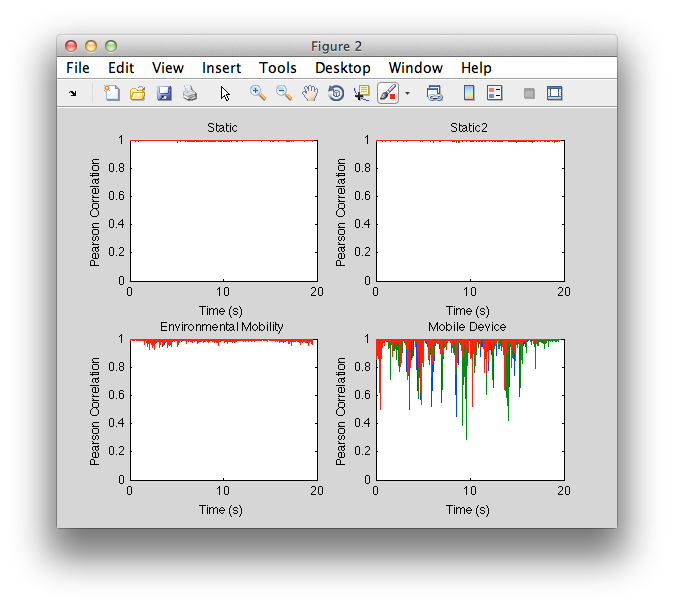
\includegraphics[width=\textwidth]{figures/esnr/mobility_csi.png}
	\caption{\label{fig:mobility_csi}CSI variation as measured by correlation in different mobility scenarios.}
\end{figure}
\begin{figure}[htp]
	\centering
	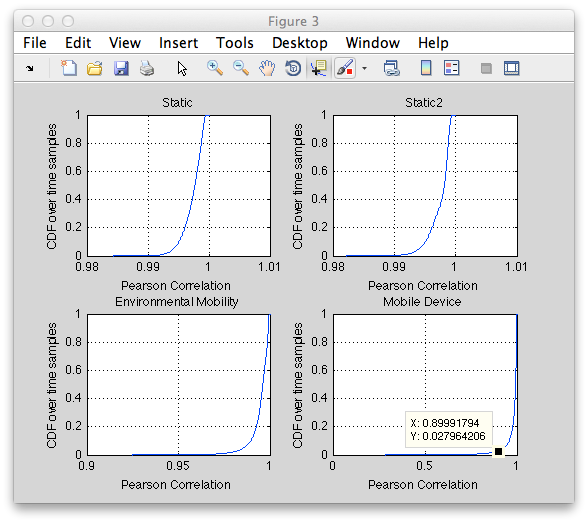
\includegraphics[width=\textwidth]{figures/esnr/mobility_csi_cdf.png}
	\caption{\label{fig:mobility_csi_cdf}CDF of CSI variation as measured by correlation in different mobility scenarios.}
\end{figure}

%%%%%%%%%%%%%%%%%%%%%%%%%%%%%%%%%%
\ifx\mainfile\undefined
%
% ==========   Bibliography   ==========
%
%\nocite{*}   % include everything in the uwthesis.bib file
\bibliographystyle{plain}
\bibliography{dhalperi_thesis}

\end{document}
\fi